
%(BEGIN_QUESTION)
% Copyright 2005, Tony R. Kuphaldt, released under the Creative Commons Attribution License (v 1.0)
% This means you may do almost anything with this work of mine, so long as you give me proper credit

Bestem hvordan utgangsresponsen blir når en konstant DC-spenning legges på inngangen til disse (ideelle) kretsene:

$$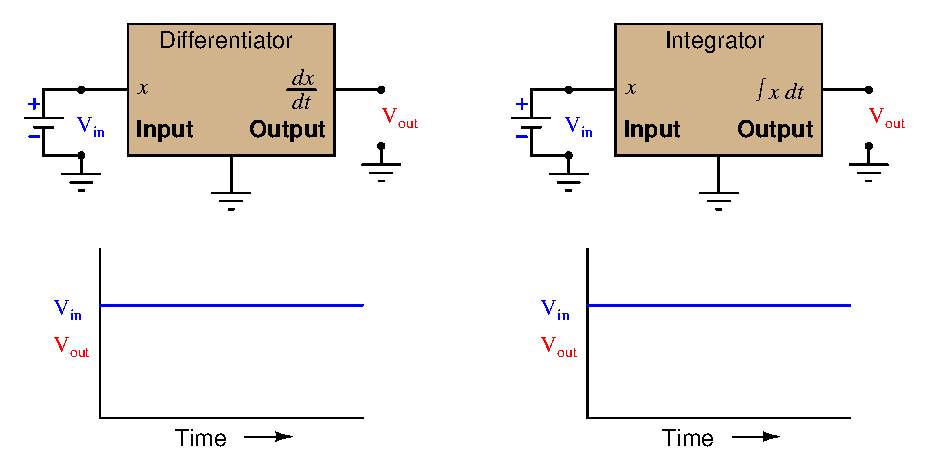
\includegraphics[width=15.5cm]{i01562x01.eps}$$

\vskip 20pt \vbox{\hrule \hbox{\strut \vrule{} {\bf Forslag til sokratisk diskusjon} \vrule} \hrule}

\begin{itemize}
\item{} Identifiser praktiske anvendelser i industrien for slike kretser.
\item{} Forklar hvordan hver av disse kretsene vil respondere på et firkantsignal med konstant frekvens.
\item{} Forklar hvordan hver av disse kretsene vil respondere på et firkantsignal med økende frekvens.
\item{} Forklar hva som skjer hvis utgangen fra integratoren kobles til inngangen på deriveringskretsen, og deretter et signal legges inn i integratoren. Hvilken type signal kommer ut av deriveringskretsen?
\item{} Forklar hva som skjer hvis utgangen fra deriveringskretsen kobles til inngangen på integratoren, og deretter et signal legges inn i deriveringskretsen. Hvilken type signal kommer ut av integratoren?
\end{itemize}

\underbar{file i01562}
%(END_QUESTION)





%(BEGIN_ANSWER)

$$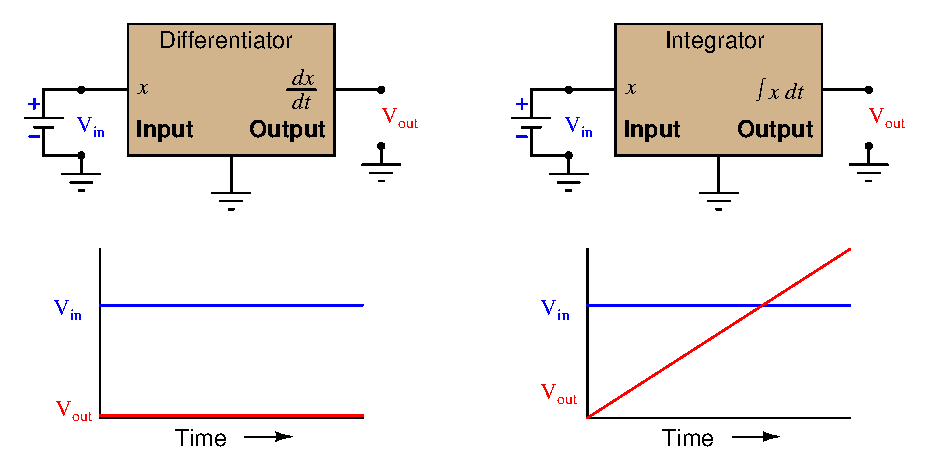
\includegraphics[width=15.5cm]{i01562x02.eps}$$

%(END_ANSWER)





%(BEGIN_NOTES)

Be studentene sette svarene inn i en praktisk kontekst, for eksempel hastighet og avstand for et objekt i bevegelse (der hastighet er tidsderivert av avstand, og avstand er tidsintegral av hastighet).

%INDEX% Electronics review: differentiator circuit response
%INDEX% Electronics review: integrator circuit response

%(END_NOTES)

